\documentclass[a4paper, 10pt, onecolumn]{report}

\usepackage[utf8]{inputenc}
\usepackage[OT1]{fontenc}
\usepackage[french]{babel}
\usepackage[dvipsnames, table]{xcolor}
\usepackage{graphicx}
\usepackage{fancyhdr}
\usepackage{calc}
\usepackage[a4paper,margin=2.5cm]{geometry}
\usepackage{array}
\usepackage{rotating}
\usepackage{hyperref}
\usepackage{makeidx}
\usepackage{listings}
\usepackage{hyperref}

\definecolor{dkgreen}{rgb}{0,0.6,0}
\definecolor{gray}{rgb}{0.5,0.5,0.5}
 
\lstset{ %
  language=C++,                % the language of the code
  basicstyle=\footnotesize,           % the size of the fonts that are used for the code
  numbers=left,                   % where to put the line-numbers
  numberstyle=\tiny\color{gray},  % the style that is used for the line-numbers
  stepnumber=1,                   % the step between two line-numbers. If it's 1, each line 
                                  % will be numbered
  numbersep=10pt,                  % how far the line-numbers are from the code
  backgroundcolor=\color{white},      % choose the background color. You must add \usepackage{color}
  showspaces=false,               % show spaces adding particular underscores
  showstringspaces=false,         % underline spaces within strings
  showtabs=false,                 % show tabs within strings adding particular underscores
  frame=single,                   % adds a frame around the code
  rulecolor=\color{black},        % if not set, the frame-color may be changed on line-breaks within not-black text (e.g. commens (green here))
  tabsize=2,                      % sets default tabsize to 2 spaces
  captionpos=b,                   % sets the caption-position to bottom
  breaklines=true,                % sets automatic line breaking
  breakatwhitespace=false,        % sets if automatic breaks should only happen at whitespace
  title=\lstname,                   % show the filename of files included with \lstinputlisting;
                                  % also try caption instead of title
  keywordstyle=\color{midnight},          % keyword style
  commentstyle=\color{dkgreen},       % comment style
  stringstyle=\color{dkgreen},         % string literal style
  escapeinside={\%*}{*)},            % if you want to add a comment within your code
  morekeywords={*,present,installed,Group,User,running,Service,Class,...}               % if you want to add more keywords to the set
}

\hypersetup{
colorlinks=true,
linkcolor=midnight,           
}

\makeindex

\begin{document}

\newcommand{\bold}[1]{\textbf{#1}}
\newcommand{\italic}[1]{\textit{#1}}
\newcommand{\surligne}[1]{\underline{#1}}
\newcommand{\couleur}[1]{\textcolor{#1}}
\newcommand{\maj}[1]{\textsc{#1}}
\newcommand{\machine}[1]{\texttt{#1}}
\newcommand{\be}{\begin{enumerate}}
\newcommand{\ee}{\end{enumerate}}
\newcommand{\bi}{\begin{itemize}}
\newcommand{\ei}{\end{itemize}}

\pagenumbering{arabic}
\xdefinecolor{midnight}{named}{MidnightBlue}
\pagestyle{fancy}
\fancyhf{}
\lhead{André Dimitri, Quentin Dexheimer et Riwan Blondé}
\rhead{\leftmark}
\rfoot{\thepage}


\begin{titlepage}

\begin{center}


\textsc{\LARGE Projet Tuteuré : \\Configuration automatique d'un cluster de calcul avec Puppet}
\vfill



\vfill

\begin{minipage}{0.99\textwidth}
\begin{flushleft} \large
André \textsc{Dimitri}\\
Quentin \textsc{Dexheimer}\\
Riwan \textsc{Blonde}\\
\end{flushleft}
\end{minipage}
\begin{minipage}{0.99\textwidth}
\begin{flushright} \large
{\large \today}
\end{flushright}
\end{minipage}


\end{center}

\end{titlepage}


% =====================================================================

\tableofcontents


\chapter{Le Grid'5000}
	\section{Présentation du Grid'5000}
	
Le Grid'5000 est une grille informatique ou grille de calcul\footnote{GLOSSAIRE !!!!grille de calcul infrastructure logicielle et matérielle qui procure à un utilisateur final un accès à des capacités de calcul et de stockage de masse hautement distribué.} destinée à la recherche scientifique, la plateforme Grid'5000 fait partie de l'action de développement technique Aladin . Le plateforme a vu le jour en 2003 et a pour but de promouvoir la recherche sur les grilles informatiques en France. Le Grid'5000 est aujourd'hui composé de 1200 noeuds répartis sur 9 sites différents situés en France et au Luxembourg et interconnectés avec le réseau Réseau National de télécommunications pour la Technologie l'Enseignement et la Recherche (RENATER). L'objectif du Grid'5000 est de permettre aux scientifiques d'effectuer des expériences dans le domaine des systèmes informatiques et des réseaux distribués dans un environnement hétérogène aussi proche de la réalité que possible.

	\begin{figure}[!h]
		\centering
   		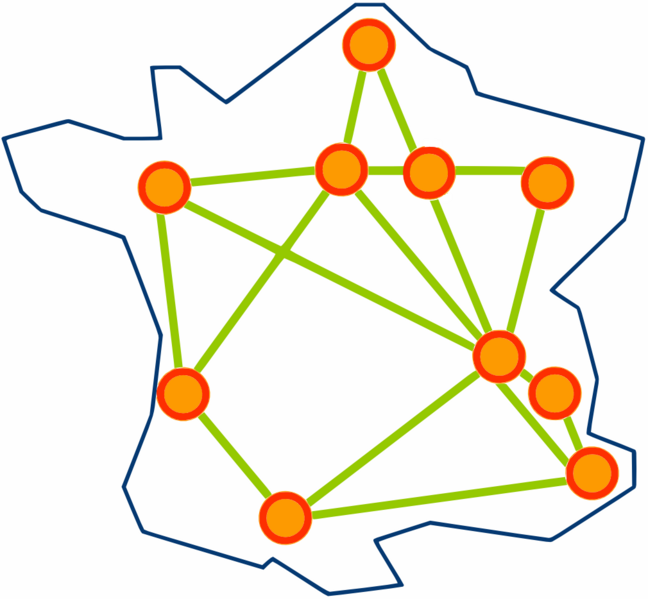
\includegraphics[width=5cm,height=5cm]{map.png}
   		\caption{Localisation des différents sites du Grid5000}
    	\label{fig:map}
	\end{figure} 

Le Grid'5000 est donc composé de plusieurs sites distincts mais l'organisation au sein de chaque site est la même. Chaque site est composé d'un ou plusieurs clusters, c'est à dire un ensemble de machine homogène.Le site de Nancy par exemple héberge deux clusters nommés Griffon et Graphene. \\
A l'intérieur de chaque cluster se trouvent des ordinateurs aussi appelés "nodes" ou "noeuds". Il existe deux types de nodes : les noeuds de services et les noeuds de travail, sur lesquels sont effectuées les expériences.\\
 Les noeuds de services servent à l'administration des machines situées dans les cluster et à l'accès aux hôtes virtuels pour les administrateurs. Les machines de services sont commune aux différents clusters situées sur les sites. Certains noeuds de services appelés "frontends" sont utilisés par les utilisateurs pour accéder aux différents sites grâce au protocole ssh, la réservation de noeuds et le déploiement. \\
L'administration de la plateforme est centralisée et est assurée par 8 personnes parmis elle certains travaille à plein temps sur la plateforme alors que d'autres non.\\
Il existe donc une hiérarchie dans la plateforme Grid'5000. Au sommet de cette hiérarchie se trouve la plateforme en elle m\^me ensuite les différents sites géographique. Au niveau inférieur on trouve les différents services et clusters puis les noeuds.  Ensuite on trouve les CPUS et enfin les cores.
	\begin{figure}[!h]
		\centering
   		\includegraphics[width=5cm,height=5cm]{griffon.jpeg}
   		\caption{Un des clusters de Nancy : Griffon}
    	\label{fig:griffon}
	\end{figure}
	
	\section{Les outils du Grid'5000}
		Le Grid'5000 est composé de plusieurs services: une partie ces services ont été développés uniquement pour cette plateforme comme par exemple Kadeploy3 qui a été developpé par l'INRIA Nancy - Grand Est; les autres sont des services standard déjà utilisés sur les systèmes Unix.  
		\subsection{OAR2}	
		\begin{figure}[!h]
			\centering
   			
\includegraphics[width=4cm,height=4cm]{oar_logo.png}
   			\caption{Le logo du projet OAR}
    		\label{fig:oar}
		\end{figure} 		
			OAR est un gestionnaire de ressources pour de grandes grilles informatique. Il est écrit en PERL et s'appuie sur une base SQL (PostgreSQL ou MySQL). OAR permet le déploiement, la réservation  et le management des noeuds et des jobs \footnote{un job correspond à une t\^ache affectée à une reservation}.\\
			Les principales fonctionnalités d'OAR sont les suivantes :  \\
			\begin{itemize}
				\item Soumission : Le système décide du moment où votre travail commence afin d'optimiser l'ordonnancement global de la plateforme. S'il n'y a pas de noeud disponible, le travail est mis en attente. (correspond à oarsub-I ou oarsub scriptName syntaxes)\\

				\item Réservation préalable: On décide alors quand le travail doit commencer, les ressources fournies seront disponibles à la date spécifiée. Si les ressources demandées sont disponibles au moment du début du job la réservation est s'effectue sinon la réservation échoue et il faut alors modifier les paramètres de la réservation. (correspond à oarsub-r date ou oarsub-R Date syntaxes scriptName)\\

				\item Mode interactif : On n'éxecute pas de script lors de la soumission ou lors de la réservation mais on choisit de travailler de facon intéractive. (correspond à oarsub-I pour la soumission ou oarsub-r jour; oarsub-C jobid pour la réservation)\\

				\item Mode passif : On choisit d'éxecuter directement un script sur les noeuds réserver. Il n'est alors pas obligatoire de se connecter sur les noeuds mais cela est toujours possible en utilisant oarsub-C jobid). (correspond à oarsub scriptName pour la soumission ou oarsub -r date scriptName pour la réservation)\\
				\item Type de job possible :  \\ \begin{itemize}
     											\item défaut: on utilise juste l'environnement par défaut des noeuds.
     											\item déployement: on déploit un système d'exploitation définis lors de la réservation. Cette méthode utilise l'outils Kadeploy.
     											\item Il existe un autre type de job , destinée aux utilisateurs avancées.
     										\end{itemize}
     		\end{itemize}
      			
		\subsection{Kadeploy3}
		
		\begin{figure}[!h]
			\centering
   			
\includegraphics[width=5cm,height=2cm]{kadeploy.jpeg}
   			\caption{Le logo du projet Kadeploy}
    		\label{fig:kadeploy}
		\end{figure} 
			Kadeploy est un outil qui permet le déploiement des différents systèmes d'exploitation sur les noeuds de la plateforme. Il permet aussi de configurer les noeuds, de les cloner et de les manager. Il permet le déploiement de système Linux, BSD, Windows et Solaris.
			
			Kadeploy3 est composé de 8 outils  : \\
				\begin{itemize}
					\item kadeploy client : l'interface utilisateur pour Kadeploy.
					\item kaenv : permet d'avoir les information concernant l'environnement des noeuds 
					\item kareboot : permet de rédemarrer les noeuds et de définir des paramètres à utiliser lors ud redemarrage.
					\item kastat : permet de connaitre les performances concernat les noeuds
					\item kaconsole : permet d'ouvrir une console sur un noeud distant.
					\item kanodes : permet de'avoir des informations copncernant les noeuds 
					\item kapower : permet  d'allumer et d'éteindre des noeuds et de connaitre le statut des noeuds (allumer/eteind)
					\item karights : permet de modifier les droits des utilisateurs sur les noeuds.
				\end{itemize}
		\subsection{Taktuk}
		\begin{figure}[!h]
			\centering
   			
\includegraphics[width=5cm,height=2cm]{TakTuk_Logo.png}
   			\caption{Le logo du projet TakTuk}
    		\label{fig:TakTuk}
		\end{figure} 
			Taktuk est un outil complémentaire à OAR2. Taktuk permet l'éxecution de commandes à distance sur un grand nombre de noeuds hétérogènes. Il met en place un liaison entre la "frontends" et les noeuds concernées par la commande et s'adapte  à l'environnement de la machine (les perfomances , la charges , le réseau ...). \\
			\surligne {Exemple :}\\ 
			\begin{lstlisting}
					taktuk -l root -s -m $puppet_master broadcast exec [ apt-get -q -y install puppet facter puppetmaster ]
			\end{lstlisting}
			L'option -l permet d'utiliser le compte root pour l'installation.\\
			L'option -m permet de déployer sur une seule machine alors que l'option -f permet de déployer sur toute les machines contenu dans le fichier.\\
			Cette commande permet donc de déployer les paquets puppet, facter et puppetmaster sur la machine puppet\_master.
			
		\subsection{KaVLAN}
			KaVLAN est un outil qui a pour but de permettre la mise en place d'un VLAN sur des noeuds du Grid5000. Il permet la mise en place de plusieurs type de VLAN : local, "router" et global. KaVLAN peut être utilisé en complément de Kadeploy et de OAR pour certains types d'expérimentation.\\
			\begin{itemize}
  				\item Un KaVLAN local est un VLAN complètement isolé du reste de la plateforme Grid5000. Il est alors obligatoire d'utiliser une gateway pour accéder aux noeuds se trouvant à l'intérieur de VLAN.
  				\item Un KaVLAN "router" permet l'accès à tous les noeuds du VLAN depuis le reste du Grid5000 sans utiliser de gateway.
 				 \item Un KaVLAN global est un VLAN qui est disponible sur tous les sites du Grid5000. Un routeur est alors configuré sur le site où le VLAN a été configuré.\\
			\end{itemize}
			\surligne {Exemple :}\\ 
			\begin{lstlisting}
					oarsub -I -t deploy -l {"type='kavlan-local'"}/vlan=1+/nodes=$nbr_nodes,walltime=$tmps -n "$nom"
			\end{lstlisting}
			La commande suivante permet de réserver un nombre donné de noeuds en utilisant un VLAN local.
			Kavlan dispose d'autres commande utile comme : \\
				\begin{itemize}
					\item La commande qui  permet d'avoir la liste des machines qui se trouvent à l'intérieur d'un VLAN pour un job donné est :
						\begin{lstlisting}
							kavlan -V -j JOBID
						\end{lstlisting}
					\item Celle qui permet d'activer le dhcp interne à KaVLAN est : 
					 	\begin{lstlisting}
							kavlan -e
						\end{lstlisting}
					\item La commande qui permet de désactiver le dhcp est : 
						\begin{lstlisting}
							kavlan -d
						\end{lstlisting}
					\end{itemize}
		\subsection{Les autres outils}
			Le Grid5000 utilise pour son fonctionnement d'autres outils :
				\begin{itemize}
					\item une base de donnée MySQL . Cette base de donnée va \^etre utilisée par Kadeploy et OAR.
					\item un serveur DNS (Domaine Name Server) qui permet de faire la correspondance entre les adresses ip et les nom de domaine.			
					\item un serveur DHCP (Dynamic Host Configuration Protocol) qui permet la configuration automatique des paramètres IP des machines.
					\item un serveur NFS (Network File System) pour permettre aux utilisateurs de stocker des informations dans leur /home sur les
 différents sites.
 					\item des  outils de supervision : \begin{itemize}
 															\item 	Nagios : surveille les hôtes et services spécifiés, alertant lorsque les systèmes vont mal et quand ils vont mieux.
 															\item 	Ganglia : permet de superviser des clusters et des grilles informatiques. 
 															\item 	Munin : présente ses résultats sous forme de graphiques disponibles via une interface web.
 															\item 	Cacti : mesure les performances réseau et serveur.
 														\end{itemize}
 					\item un serveur weathermap : qui permet la visualisation du réseau sous forme d'une carte.
 					\item un serveur syslog : qui permet les journaux d'évènements.
 					\item un annuaire LDAP ( Lightweight Directory Access Protocol) : permet le stockage d'informations et de données.
 					\item un serveur web Apache avec un proxy.
 					\item un serveur Squid :  un proxy/reverse proxy
 					\item un serveur NAT (Network Address Translation) : permet de faire correspondre une seule adresse externe publique visible sur Internet à toutes les adresses d'un réseau privé
 					\item un serveur mail.
 					\item un dep\^ots de paquets et de logiciels.
 					\item API Rest g5k : utiliser par KaVLAN, Kadeploy et UMS (User Management System). Elle permet d'utiliser toute les fonctions du Grid'5000 et de les automatiser.
 					\item une infrastructure de virtualisation XEN comportant de 2 à 5 dom0 et environ 30 domU avec un service par domU.
 					
				\end{itemize}

\begin{thebibliography}{99}
\bibitem{ref} https://www.grid5000.fr/mediawiki/index.php/Grid5000:Home
\bibitem{ref} http://kadeploy3.gforge.inria.fr/
\bibitem{ref} http://oar.imag.fr/
\bibitem{ref} http://taktuk.gforge.inria.fr/
\bibitem{Pro.puppet}
        Pro Puppet
		James Turnbull , Jeffrey McCune 
        Apress
        2011.


          
\end{thebibliography}

\end{document}
